\section{Running {YOLOv3-Tiny}}
\label{sec:example}

To demonstrate Tiny-Vedas capabilities, I elected to
run an \texttt{int8} quantized version of {YOLOv3-Tiny}~\cite{redmon2018yolov3}: a Darknet detector with
a small convolutional backbone, max-pool downsampling, a leaky {ReLU}
after each fused convolution, an upsample/concat skip, and two linear
detect heads.
The Alveo U280 runs in this paper use a $208{\times}208$ letterboxed input
(Tiny-208). The backbone of the network is offloaded to Tiny-Vedas, while the host finishes Non-Maximum Suppression ({NMS}) 
and box decode.

\paragraph{Quantization and calibration.}
The exported {PyTorch} model is an integer graph: activations travel as
\texttt{int32}, weights are \texttt{int8} values held in
\texttt{int32} containers, and each convolution is
\texttt{im2col} plus a {GEMM} {DA} call.

The {GEMM} accumulates in \texttt{int32}.
The next layer's pack needs those values in the \texttt{int8} range.
A scalar \texttt{requant\_i32} does that:
\begin{equation*}
  y=\mathrm{clamp}((x{\cdot}\mathrm{mul}){\gg}\mathrm{shift},-127,127).
\end{equation*}
Figure~\ref{fig:yolo-stage} is one repeating stem stage.

\begin{figure}[H]
  \centering
  \setlength{\intextsep}{4pt}%
  % One repeating Tiny-208 stem stage (integer graph). Compact: must
% fit under its first cite in a short column.
\definecolor{tvink}{HTML}{111111}
\definecolor{tvmute}{HTML}{333333}
\definecolor{tvline}{HTML}{555555}
\definecolor{tvshade}{HTML}{EEEEEE}

\begin{tikzpicture}[
  >=Stealth,
  x=1mm, y=1mm,
  font=\sffamily\scriptsize,
  box/.style={
    draw=tvink,
    line width=0.55pt,
    rounded corners=1.2pt,
    fill=white,
    align=center,
    inner xsep=1.4pt,
    inner ysep=1.4pt,
    font=\sffamily\tiny,
    minimum height=7.2mm,
  },
  hub/.style={
    box,
    line width=1.0pt,
    fill=tvshade,
    font=\sffamily\tiny\bfseries,
  },
  arr/.style={
    ->,
    draw=tvline,
    line width=0.5pt,
    shorten >=0.6pt,
    shorten <=0.6pt,
  },
]
\pgfmathsetmacro{\W}{\columnwidth/1mm - 0.8}

\draw[tvink, line width=0.55pt, rounded corners=1.6pt]
  (0, 0.2) rectangle (\W, 16.4);

\node[font=\sffamily\tiny, text=tvmute, anchor=east] (xin)
  at (0.07*\W, 8.3) {int32};
\node[box, anchor=west] (conv) at (0.09*\W, 8.3)
  {\textbf{Conv}\\[0.05em]
   {\color{tvmute}\ttfamily\tiny im2col+GEMM}};
\node[box] (leaky) at (0.42*\W, 8.3)
  {\textbf{Leaky ReLU}\\[0.05em]
   {\color{tvmute}\ttfamily\tiny Zve32x}};
\node[hub] (rq) at (0.66*\W, 8.3)
  {\texttt{requant\_i32}\\[0.05em]
   {\normalfont\color{tvmute}\ttfamily\tiny (mul, shift)}};
\node[box] (pool) at (0.88*\W, 8.3)
  {\textbf{Max-pool}\\[0.05em]
   {\color{tvmute}\ttfamily\tiny Zve32x}};

\draw[arr] (xin) -- (conv);
\draw[arr] (conv) -- (leaky);
\draw[arr] (leaky) -- (rq);
\draw[arr] (rq) -- (pool);

\end{tikzpicture}

  \caption{One stem stage: \texttt{im2col}+{GEMM}, leaky {ReLU},
    \texttt{requant\_i32}, max-pool.
    Detect heads drop the leaky and the pool.}
  \label{fig:yolo-stage}
\end{figure}

The pair $(\mathrm{mul},\mathrm{shift})$ is per layer: each layer has
its own dynamic range.

Calibration chooses those pairs offline.
An {FP32} run of the same net measures per-layer activation scales;
I pick $(\mathrm{mul},\mathrm{shift})$ so
$\mathrm{mul}/2^{\mathrm{shift}}\approx
\mathrm{scale}_x{\cdot}\mathrm{scale}_w/\mathrm{scale}_y$,
and I rewrite the bias into accumulator units.
That maps most layers onto $[-127,127]$;
the detect heads keep $\mathrm{scale}_y{=}1$ and stay in logit units.
The formula uses one $\mathrm{scale}_w$ for the whole layer.
Per-channel weight scales are the obvious alternative: each output
channel keeps its own range.
Then $\mathrm{scale}_x{\cdot}\mathrm{scale}_w/\mathrm{scale}_y$ would
differ by channel, and \texttt{requant\_i32} would need a
$(\mathrm{mul},\mathrm{shift})$ per channel.
I left the operator scalar---one multiply and one shift for the
map---so the weights share one scale.
A per-channel requant would mean a vector of pairs in the operator,
the calibration file, and codegen; I did not grow the kernel.

The pairs go into a calibration file that \pyv{} loads
(Figure~\ref{fig:requant-cal}).
Since calibration is ubiquitous on quantized models, I added native
calibration support to PyVedas through calibration files.

\begin{figure}[H]
  \centering
  % Column-width excerpt of the requant calibration file (schema, not a run).
\definecolor{tvink}{HTML}{111111}
\definecolor{tvmute}{HTML}{333333}

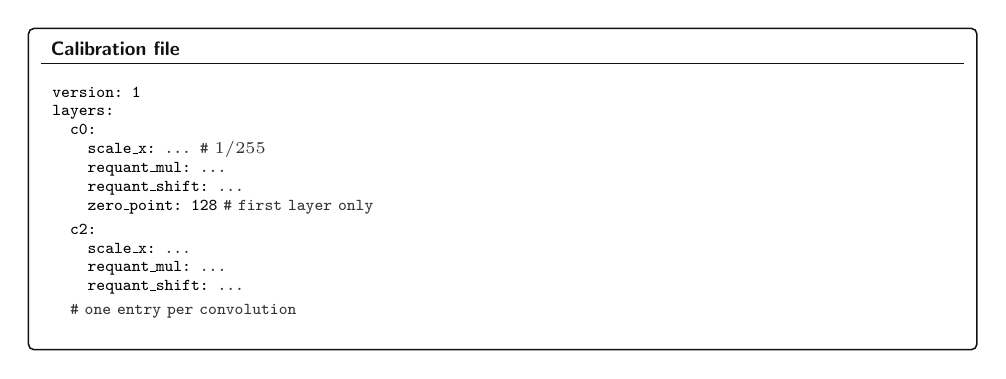
\begin{tikzpicture}[
  x=1mm, y=1mm,
  font=\sffamily\tiny,
]
\pgfmathsetmacro{\W}{\columnwidth/1mm - 0.8}

\draw[tvink, line width=0.55pt, rounded corners=2pt]
  (0, -0.8) rectangle (\W, 40.0);

\node[font=\sffamily\scriptsize\bfseries, text=tvink, anchor=west]
  at (1.6, 37.4) {Calibration file};
\draw[tvink, line width=0.4pt]
  (1.6, 35.5) -- (\W-1.6, 35.5);

\node[
  anchor=north west, align=left,
  font=\ttfamily\fontsize{5.6}{6.8}\selectfont,
  text width=0.90*\columnwidth
] at (1.8, 33.8) {%
version: 1\\
layers:\\
\quad c0:\\
\quad\quad scale\_x: \textcolor{tvmute}{\ldots}
  \textcolor{tvmute}{\# $1/255$}\\
\quad\quad requant\_mul: \textcolor{tvmute}{\ldots}\\
\quad\quad requant\_shift: \textcolor{tvmute}{\ldots}\\
\quad\quad zero\_point: 128
  \textcolor{tvmute}{\# first layer only}\\[0.3em]
\quad c2:\\
\quad\quad scale\_x: \textcolor{tvmute}{\ldots}\\
\quad\quad requant\_mul: \textcolor{tvmute}{\ldots}\\
\quad\quad requant\_shift: \textcolor{tvmute}{\ldots}\\[0.3em]
\quad \textcolor{tvmute}{\# one entry per convolution}%
};

\end{tikzpicture}

  \caption{Calibration file: one layer entry with
    $\mathrm{scale}_x$ and the $(\mathrm{mul},\mathrm{shift})$ pair.
    \pyv{} loads it; the compiler does not embed the scales.}
  \label{fig:requant-cal}
\end{figure} 

\paragraph{Data tiling.}
A Tiny-208 layer's activations and \texttt{im2col} buffers do not
always fit in {DCCM}.
The {JIT} therefore cuts spatial and output-channel tiles so the live
working set stays on chip, and moves whatever still does not fit
through the 16\,mebibyte ({MiB}) {SRAM} stub at \mbox{\texttt{0x40000000}}.
After a few iterations I landed on \texttt{cache\_col}.
It writes one \texttt{im2col} panel per spatial tile into {DCCM},
then walks output channels: pack a weight tile once, and reuse
every cached panel.
On Tiny-208 \texttt{c12} that is six \texttt{im2col} buffers and
256 packs.

The {SRAM} stub is a placeholder:
the same window can later be a shared level-2 ({L2}) cache from
several \tv{} cores into High Bandwidth Memory ({HBM}), the way a
{GPU} {SoC} is built.

\paragraph{GEMM tiling.}
Separately, every Tiny-208 convolution lowers to a matrix multiply
whose $M$, $N$, and $K$ are far larger than $8{\times}8$ with
$K{=}32$---early layers have tens of thousands of output pixels;
deep layers have $K$ in the thousands.
\pyv{} cuts that multiply into tiles $(m_t,n_t,k_t)$ that fit one
hardware job, and emits nested loops: each iteration packs a slice,
rings {START}, and writes its piece of $C$.

Division of labor inside the binary is simple.
Convolution hits the {GEMM} over {MMIO}.
Leaky {ReLU} and max-pool stay on {Zve32x}
(\texttt{vsetvli} e32/m1, \texttt{vle32}/\texttt{vse32},
\texttt{vmax}/\texttt{vmin}).

Figure~\ref{fig:card-det} is the closed loop: letterbox on the host,
backbone on the card, boxes back on the host.
The numbers that prove it closed are in \S\ref{sec:eval}.

\begin{figure}[H]
  \centering
  
\includegraphics[width=0.92\linewidth]{card_000000000009.jpg}
  \caption{One Tiny-208 frame on the card: backbone {ELF}, host {NMS},
    192 boxes (12 drawn).}
  \label{fig:card-det}
\end{figure}
